\documentclass{NSF}
\usepackage{amssymb}
\usepackage{graphicx}
\graphicspath{ {images/} }

\begin{document}
% B. Project Summary
\title{Computer Science Capstone: Lifting Squares to a Half-space, a Specific Case of Lifting Pseudo-disks}
\newsection{Project Progress Report}
\section{Myunggun Seo}
\section{Project Summary}

\subsection{Abstract}
% Your short version of your proposal goes here
A \textbf{hypergraph} $H = (V, E)$ consists of the base set $V$, called hypervertices and consisting of vertices and a set $E$, called hyperedges. Hypervertices are the equivalent of a graph's vertex in a hypergraph. The set $E$ is a subset of the powerset of $V \times V$. In other words $E$ contains some subsets of $V$. A \textbf{support} graph or \textbf{support} $S = (V_S, E_S)$ of a hypergraph $H = (V_H, E_H)$ is a graph with the same vertex set as $H$, ie. $V_S = V_H$, in which the subgraph $G_e = (e, E_S \cap e \times e)$ of $H$ induced by each hyperedge $e \in E$ is a connected graph. Our problem is: for a given hypergraph, represented as a set of regions in a simple closed Jordan curve $\mathcal{R} = \{ R_1, ... , R_n \}$, build a planar graph $G$ on $R$ such that for each $p \in \mathbb{R}^2$, the set $\{R \in \mathcal{R} : p \in R\}$ forms a connected subgraph of $G$. 

\subsection{Introduction: General Case of Pseudo-disks}
The problem that we tackle is a specific case of an unsolved problem in computational geometry: Given a set of pseudo-disks $\{D_i\}$ and points $\{P_j\}$ in $\mathbb{R}^2$ in arbitrary positions, is there a mapping from the pseudo-disks and points to a set of half-spaces $\{H_i\}$ and points $\{Q_j\}$ in $R^3$ such that the membership of point $P_j$ in a pseudo-disk $D_i$ is preserved with point $Q_j$ in $H_i$? If there is, what is the mapping?

\subsection{Appendix: Definitions}

Pseudo-disks are a set of closed Jordan curves in $\mathbb{R}^2$ in which any pair of pseudo-disks intersect at maximum two places. This property is derived from disks in $\mathbb{R}^2$.

A half-space in $\mathbb{R}^3$ is either of the two parts separated by a plane. In general, a half-space is either of the two parts divided by a hyperplane in a $\mathbb{R}^k$.

\subsection{Hypergraphs}



For this research we consider \textbf{undirected graphs} where the order of vertices in an edge does not matter, ie. $e = (v,w) = (w,v)$ for $e$ in $E$ of graph $G = (V, E)$. $G' = (V', E')$ is a \textbf{subgraph} of graph $G = (V, E)$ if $V' \subseteq V$ and $E' \subseteq E$. Also, $G'$ is the vertex-induced subgraph (\textbf{induced subgraph}) of $G$ if $E' = E \cap (V' \times V') $. Verbally, an induced subgraph of a graph is a subgraph that has all of the edges of the original graph that connects each and every vertex in the subgraph.   \\



A \textbf{hypergraph} $H = (V, E)$ consists of the base set $V$, called hypervertices and consisting of vertices and a set $E$, called hyperedges. Hypervertices are the equivalent of a graph's vertex in a hypergraph. The set $E$ is a subset of the powerset of $V \times V$. In other words $E$ contains some subsets of $V$. Formally, $E \subseteq \mathcal{P}(V)\backslash\emptyset$ where $\mathcal{P}(V)$ is the powerset of $V$. \\

The difference between a graph and a hypergraph is that a graph's edges connect two vertices each. Geometrically, an edge can be drawn as an edge but we can see also the edge as a set of two vertices. In a hypergraph, we expand the definition of an edge as a set of any positive number of vertices. The notion of vertices remain the same in hypergraphs.\\

% \subparagraph{Representations of Hypergraphs} 
There are multiple ways to represent a hypergraph. Having multiple representations is useful in thinking creatively from multiple perspectives. As such, different representations have been used to derive proofs and explanations for support graphs because each depiction has a relationship with the support graph. Here we discuss a few.

\begin{figure}[ht]
\centering
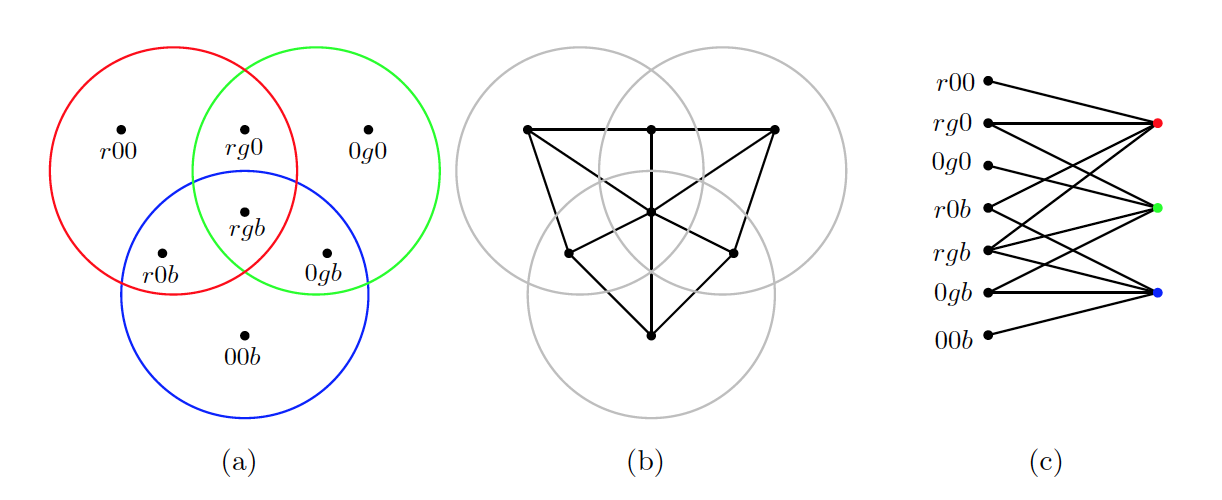
\includegraphics[width=\textwidth]{diagram1}
\caption{Three different representations of hypergraphs: (a) an Euler Diagram of a hypergraph where each Jordan curve represents a hyperedge. For this instance, it is identical to the Venn Diagram (b) the dual of the Euler Diagram which is always a support, and (c) the incidence graph which is a bipartite graph of the vertices on one side and the hyperedges on the other. (Source: Bruckdorfer \cite{tubingen2016})}
\end{figure}

\subparagraph{Euler Diagram}
In an Euler diagram, each hypervertex is shown as a point in the plane and each hyperedge is drawn as a simple closed Jordan curve that encloses all the hypervertices that the hyperedge contains. Figure 1.a depicts an Euler diagram representation of the hypergraph with $V = \{r00, rg0, 0g0, r0b, rgb, 0gb, 00b\}$ and $E = \{  \{r00,rg0,rgb,r0b\}, \{rg0,0g0,rgb,0gb\}, \{r0b,rgb,0gb,00b\}  \}$. This is visually similar to a Venn diagram where we would need to draw all $2^n$ possible regions for $n$ hypervertices even if there are no corresponding hyperedges to some regions. Note that as the hyperedges become more sizable and complex, it becomes harder to draw the Euler Diagram in an elegant manner. The Euler Diagram is also similar in structure to the Intersection Structure drawing or the Hasse Diagram.

\subparagraph{Support of Hypergraph}
Hypergraphs can also be represented with its support.

In Figure 1.b, the support is the dual graph of the Euler Diagram. However, there can be multiple supports for a given hypergraph and thus a support need not be the dual of the Euler Diagram. 
The fact that there can be multiple supports means that sometimes supports do not give all the information for how the hypergraph looks like.



\subparagraph{Incidence Graph}
The incidence graph is a bipartite graph that represents hypervertices as one group of vertices of the graph and hyperedges as another. If a hypervertex is in a hyperedge, there is an edge in the incidence graph. Figure 1.c is an example of an incidence graph.
The structure of an incidence graph is much simpler than the Euler diagram. However, because each hyperedge-hypervertex edge lacks identifiability, it is harder to recognize the overall structure compare to an Euler diagram.

\subparagraph{Dual of Hypergraph}
From the Incidence graph, we can see that it is easy to swap the position of hypervertices and hyperedges. As with graphs, the notion of a dual is defined as follows: a dual $G'$ of a hypergraph $G$ is a hypergraph with $E_G$ as its hypervertices and $V_G$ as its hyperedges. In an incidence graph representation, a hypergraph and its dual will have a symmetric layout.

Johnson and Pollak \cite{johnson1987} showed that a hypergraph with a tree support has an acyclic hypergraph as its dual. Acyclicity can be checked in linear time.


\subparagraph{Matrix Representation}
Hypergraphs can be mapped to a matrix $M$ of size $n\times m$, where the columns represent the $m$ hypervertices and the rows represent the $n$ hyperedges. If the $i$th hypervertex is an element of the $j$th hyperedge, $M_{ij} = 1$ and 0 otherwise. Korach and Stern showed that the problem of finding path supports is equivalent to finding a permutation of the columns of $M$ such that each row has consecutive 1's. Tucker showed that the problem of finding cycle supports in equivalent to finding a permutation such that each row of $M$ has circularly consecutive 1's.

\subparagraph{Intersection Structure, Connectivity Structure, and Hasse Diagram}
The intersection structure is a directed graph with all possible intersections of 1 or more hyperedges as the vertices. There is an edge from one vertex $v1$ of this graph to another $v2$ if $v1 \subset v2$ but $\nexists v3$ s.t. $v1 \subset v3 \subset v2$. In other words, the intersection structure demonstrates the hierarchy of subsets that form the original hyperedges. Another name for the intersection structure is the Hasse Diagram. 

A \textit{demand} of a vertex in the intersection structure is the number of additional elements required on top of the union of its subsets.


\begin{figure}[ht]
\centering
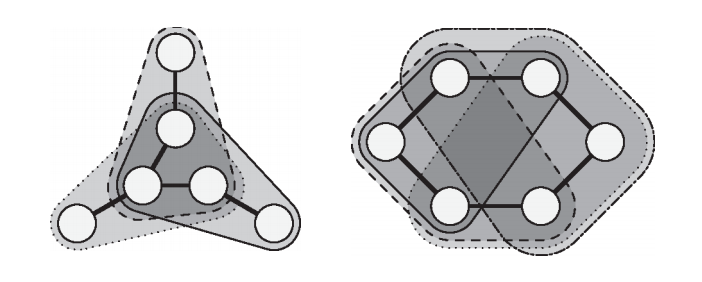
\includegraphics[width=\textwidth]{optimal-hypergraphs}
\caption{Examples of minimum supports. The hypergraph is represented with white nodes as hypervertices and hyperedges as gray areas. The support is the graph with white nodes and black edges connecting white nodes. (Source: Chen et al. \cite{Chen2015}) }
\end{figure}


\subsection{Supports}
A \textbf{support} graph or \textbf{support} $S = (V_S, E_S)$ of a hypergraph $H = (V_H, E_H)$ is a graph with the same vertex set as $H$, ie. $V_S = V_H$, in which the subgraph $G_e = (e, E_S \cap e \times e)$ of $H$ induced by each hyperedge $e \in E$ is a connected graph. Recall that each hyperedge $e$ is a set of vertices. In other words, a support graph of a hypergraph is able to "support" each of the hyperedges by keeping all the hypervertices in a hyperedge connected.
A planar support of a hypergraph is a support that can be drawn without overlapping edges.\\

Figure 2 shows two examples of support graphs of hypergraphs. Whichever hyperedge (grey region enclosed by black curve) you look at, all the vertices in that hyperedge is connected. If you remove any edge (black line connecting the white vertices), not all induced subgraphs of hyperedges are connected. Thus these are examples of minimal supports. In fact, they are minimum supports for the given hypergraphs.


\subsection{Problem Statement}
Thus our problem can be formally stated as:\\
For a given hypergraph, represented as a set of regions in a simple closed Jordan curve $\mathcal{R} = \{ R_1, ... , R_n \}$, build a planar graph $G$ on $R$ such that for each $p \in \mathbb{R}^2$, the set $\{R \in \mathcal{R} : p \in R\}$ forms a connected subgraph of $G$. 


Chen et al. \cite{Chen2015} gave an overview of the history and status quo of research around support graphs. They analyze multiple different research fields and concludes that the following problems that are the same problem of finding Supports of Hypergraphs:
\begin{enumerate}
\item Subset Interconnection Design Problem (SID)
\item Minimum Topic-Connected Overlay
\item Interconnection Graph Problem
\item Network Inference
\item Host graphs
\item Spanning graphs
\item Support (only certain structures)
\end{enumerate}
Such different names arose from different research fields  \cite{Chen2015}


\subsection{Specific Goals}

This research project will not aim at completely solving the problem of finding planar supports of hypergraphs but at solving several specific sub-problems that will help gain a greater understanding of the problem or novel ways to approach it.\\

Here I propose a few feasible sub-problems that this research project will attempt to solve.
\begin{enumerate}
\item Determine if 1-outer planar support exists for general hyperedges
\item Assuming that a planar support of a given hypergraph exists, how can we efficiently find an approximation such as a $k$-planar graph? 
\item Find a planar support of a hypergraph where the shapes of the regions are restricted to rectangles, disks, or arbitrary shapes that have at most $k$ number of intersections with other regions.
\item Given k-piercing regions (defined as regions pierced by maximum or on average k other regions), can we find a planar support?
\item Continue on Chen et al.'s work of varying the following parameters: 
size $d$ of the largest hyperedge, 
number $m$ of hyperedges in hypergraph,
feedback edge number $\phi = k-n+1$ of the solution -- this is a measure of sparseness where $k=$ number of edges in the solution and $n=$ number of vertices in original hypergraph.
\end{enumerate}

% Your Literature Review
\subsection{Related Work}
% Give an overview of the current state of knowledge on the particular topics. Include competing ideas and hypotheses as well as the major lines of evidence supporting or not supporting the different hypotheses. 
%Describe related work. All citations in your bibliography must be referenced in your proposal.

Johnson and Pollak proved that it is NP-complete to decide if a given hypergraph has a planar support.
Buchin et al. proved that it is NP-complete to decide whether a hypergraph has a 2-outerplanar support and that it is NP-hard to decide if a hypergraph has a 3-outerplanar support. \cite{buchin2010}
% (A k-outerplanar graph is a graph that can be drawn in the plane without crossing such that after k-fold removal of the vertices on the outer-face there are no vertices left. https://www.sciencedirect.com/science/article/pii/S0166218X1400434X)

In contrast, there are polynomial time algorithms to test whether a given hypergraph has a planar support that is a path, cycle, or tree. \cite{johnson1987}
Ray proved that for non piercing regions there is always a planar support and the proof provides an algorithm in $O(n^3)$ time complexity. \cite{Pyrga2008}
If the set of hyperedges is closed under intersections and differences, it can be decided in polynomial time whether the hypergraph has a planar or outerplanar support. \cite{brandes2011}

Finding the minimum support of special structures is also of interest in some fields.
It is known that finding the minimum weight support is NP-hard. \cite{Du1998}
There have been efforts to approximate minimum support using genetic algorithms \cite{abuali1996} and polynomial time greedy algorithms. \cite{Du1998}

Under certain circumstances, the minimum support can be found in polynomial time.
A minimum weighted tree support can be computed in polynomial time. \cite{Korach2003} Buchin et al. also showed that a support with the minimum number of edges can be computed in polynomial time if the hypergraph is closed under intersections. \cite{buchin2010}


\subsection{Potential Impact}
% Describe why the proposed research is important.
% Provide a statement of what you think the impact of your research will be. Be as specific as possible. 

The goal of this research project is to contribute to the ongoing theoretical discussion of planar supports and is not necessarily motivated by applications. However, there exist multiple uses of the outcome of this research project, especially in visualizing big sets \cite{meulemans2013} or colored graphs \cite{hurtado2017}. In some cases, supports are used for Social Network Theory.

It is also a subproblem of the NP-hard Subset Interconnection Design problem, also known as Minimum Topic-Connected Overlay. This problem has many applications in design of scalable overlay networks, vacuum systems, reconfigurable interconnection network, etc. \cite{Chen2015}



\subsection{Methodology}
% Describe the approach and methodology you want to pursue in order to achieve the capstone goal and/or answer the research question.

This research will generally consist of iteration of the following process. Visualize the problem. Find mathematical proofs. Provide experimental evidence via programming. Branch the problem into more easily solvable problems. 

Depending on the nature of a sub-problem, I will also employ software to brute-force solutions or to create visual representations of hypergraphs and their supports in the different methods noted above.

  
\subsection{Budget}
% Give a financial budget listing the type and cost of the necessary equipment, materials, supplies, experiments, etc. with justifications for each. NYUAD has allocated a maximum financial support of 2,000 U.S. Dollars for each capstone research project, so your budget should fall within this limit. 

This project is mainly theory-based and thus will require wide writing space for ideation and sharing ideas with my team-mate. 

\begin{itemize}
\item Whiteboard (90cm$\times$120cm): 1 pcs $\times$ 50 USD $=$ 50 USD 
\item Markers (4 markers/box) : 12 pcs $\times$ 10 USD $=$ 120 USD 
\item Whiteboard Eraser : 2 pcs $\times$ 5 USD $=$ 10 USD
\item Whiteboard Cleaner Fluid : 1 pcs $\times$ 8 USD $=$ 8 USD
\end{itemize}

This will amount to a total of 188 USD.



\renewcommand\refname{References}
\bibliography{references}
% The IEEE bibliography style is NOT rBibliography listing all cited references.
% Feel free to use whatever style you prefer
\bibliographystyle{IEEEtran}

\end{document}

